\chapter{Desenvolvimento/procedimento}
\label{ch:desenvolvimento}

Para o desenvolvimento do robô, foi necessário desenvolver o modelo \textit{CAD}, a criação do modelo físico em \textit{CoppeliaSim}, a implementação de código em \textit{Matlab} e ainda a comunicação entre o \textit{CoppeliaSim} e \textit{Matlab}. Relativamente à parte de desenvolvimento do modelo \textit{CAD} do robô, conceberam-se diversas peças desde a sua raiz e foram ajustadas peças já concebidas. Por outro lado, adaptou-se código para controlo do robô, nomeadamente para se desviar de obstáculos e atingir um alvo. De modo a ser possível controlar o robô foram ajustados diversos parâmetros posteriormente testados.
%
%
%
\section{\textit{Autodesk Fusion 360}}
\label{sec:autodesk}

No desenvolvimento do modelo CAD do robô foram concebidas diversas peças: uma base, uma prateleira, uma tampa, uma bateria e quatro suportes. Para além destas peças, foram escolhidas peças já desenvolvidas: duas rodas motrizes, duas rodas giratórias, dois motores e doze sensores. Após todas as peças desenvolvidas e ajustadas, foi feito o assembler das diversas peças formando assim o robô. De seguida, é possível visualizar os desenhos técnicos de cada peça, a peça em modelo CAD e uma breve descrição de cada peça:

\begin{itemize}
    \item \emph{Base:} Projetou-se uma base cilíndrica com 1cm de altura e 15 cm de raio. Esta base serve de suporte a todo o robô e têm um encaixe para os motores (Figura \ref{fig:base}).
    %
    \begin{figure}[!h] 
\centering
    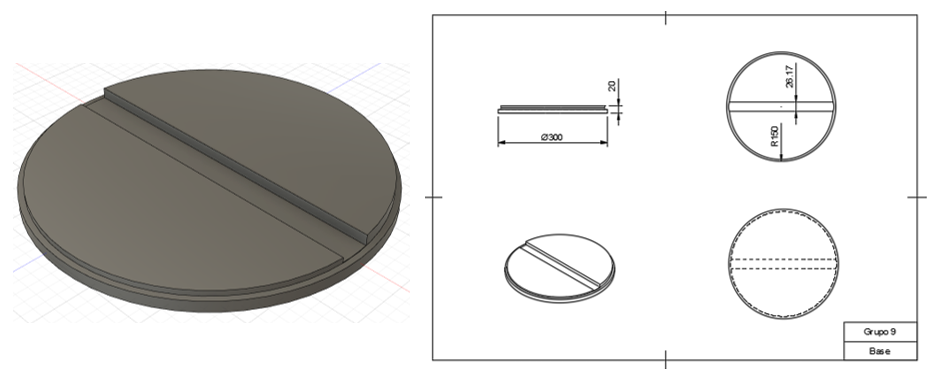
\includegraphics[width=0.7\textwidth]{./img/base}
  \caption{Base do robô}% 
\label{fig:base}
\end{figure}

    \item \emph{Prateleira:} Foi desenvolvida uma prateleira com 9 cm de altura, para criar duas divisões na base. Sendo a divisão inferior para a colocação dos motores e fios necessários e na divisão superior é colocada bateria. Esta prateleira serve para isolar todos os elementos que estão apoiados na base do exterior conferindo uma maior segurança dos mesmos (Figura \ref{fig:prateleira}).
    %
    \begin{figure}[!h] 
\centering
    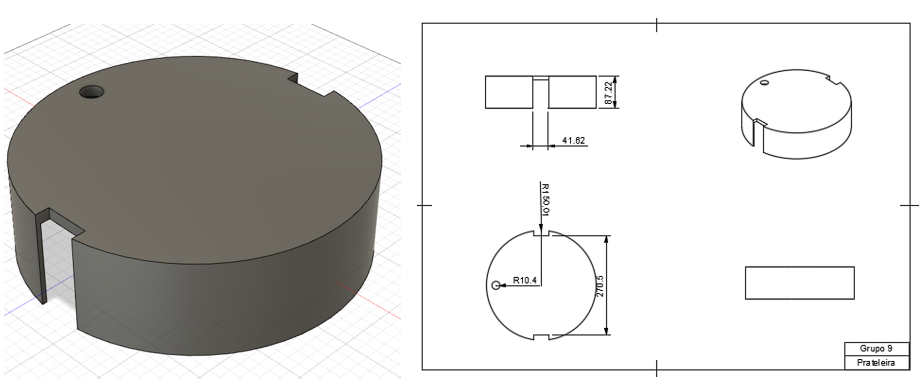
\includegraphics[width=0.65\textwidth]{./img/prateleira}
  \caption{Prateleira do robô}% 
\label{fig:prateleira}
\end{figure}

    \item \emph{Tampa:} Elaborou-se uma tampa com 2cm de altura e um raio de 15 cm, para que esta fique apoiada nos suportes. Esta tampa é a camada mais alta do robô e protege os elementos que estão abaixo dela (Figura \ref{fig:tampa}).
        %
    \begin{figure}[!h] 
\centering
    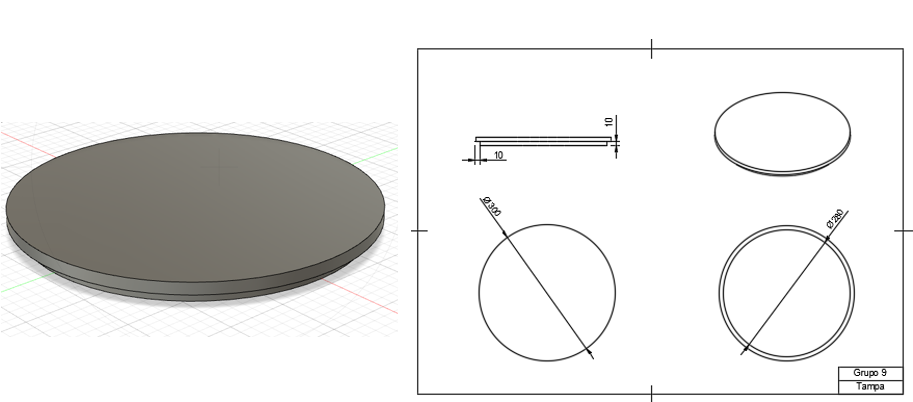
\includegraphics[width=0.65\textwidth]{./img/tampa}
  \caption{Tampa do robô}% 
\label{fig:tampa}
\end{figure}

\item \emph{Suportes:} Para dar altura ao robô de forma a colocar alguns elementos fora do interior do robô foram criados 4 suportes (Figura \ref{fig:suportes}).
        %
    \begin{figure}[!h] 
\centering
    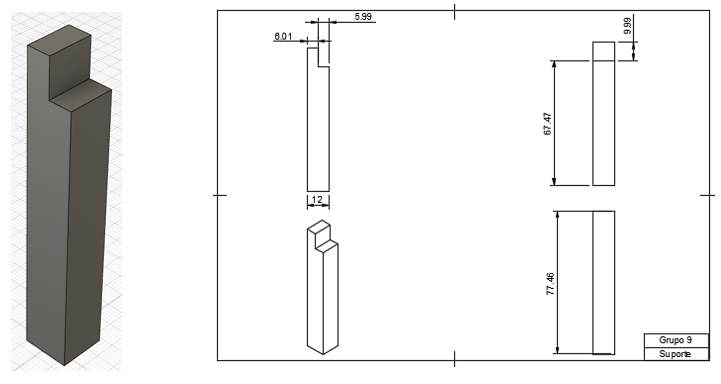
\includegraphics[width=0.6\textwidth]{./img/suportes}
  \caption{Suportes do robô}% 
\label{fig:suportes}
\end{figure}

\item \emph{Sensores:} O modelo do robô possui 12 sensores infravermelhos previamente concebidos, nos quais foi necessário ajustar as medidas. Estes estão igualmente espaçados entre si ao redor de toda a base. Estes sensores têm um alcance de 80 cm e uma amplitude de 30º (Figura \ref{fig:sensores-2}).
        %
    \begin{figure}[!h] 
\centering
    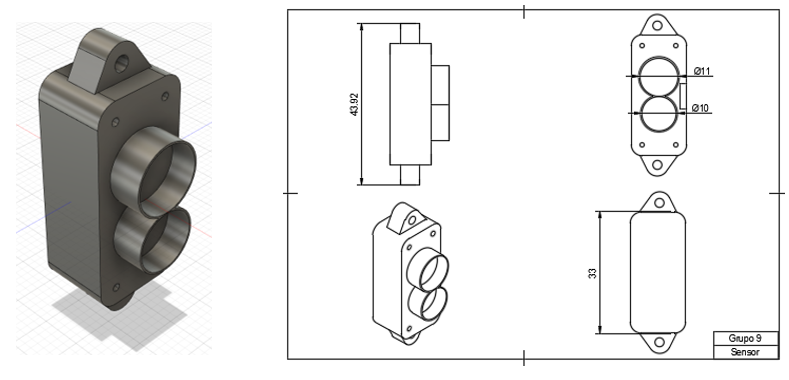
\includegraphics[width=0.6\textwidth]{./img/sensores-2}
  \caption{Sensores do robô}% 
\label{fig:sensores-2}
\end{figure}

\item \emph{Bateria:} : Foi desenvolvida uma bateria com 15 cm de comprimento, 10,5 cm de altura e 6,5 cm de largura. A bateria foi desenhada com base em modelos reais. Para fazer a bateria, foi desenhado um retângulo com 15 x 6,5 cm, utilizando a ferramenta \textit{Create Sketch}, de seguida, através da ferramenta extrude foi dada uma altura de 10,5 cm, conferindo-lhe assim a forma de paralelepípedo. Após isto feito, foi desenho um novo retângulo no topo do paralelepípedo e novamente através da ferramenta extrude foi removido o centro do retângulo de forma a criar os terminais que se encontram na parte de cima da bateria como é vísivel na figura seguinte (Figura \ref{fig:bateria}).
        %
    \begin{figure}[!h] 
\centering
    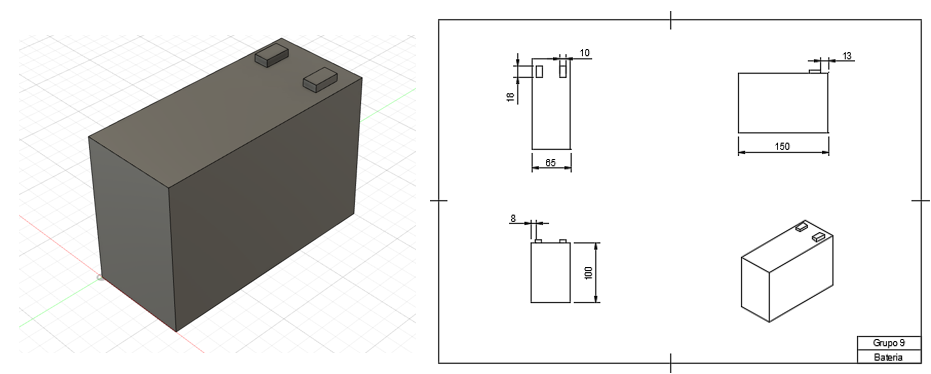
\includegraphics[width=0.8\textwidth]{./img/bateria}
  \caption{Bateria do robô}% 
\label{fig:bateria}
\end{figure}

\item \emph{Motor:} O modelo do robô possui dois motores 12V DC. Foi utilizado um design já concebido, sendo depois necessário adaptar às características do nosso robô (Figura \ref{fig:motor}).
        %
    \begin{figure}[!h] 
\centering
    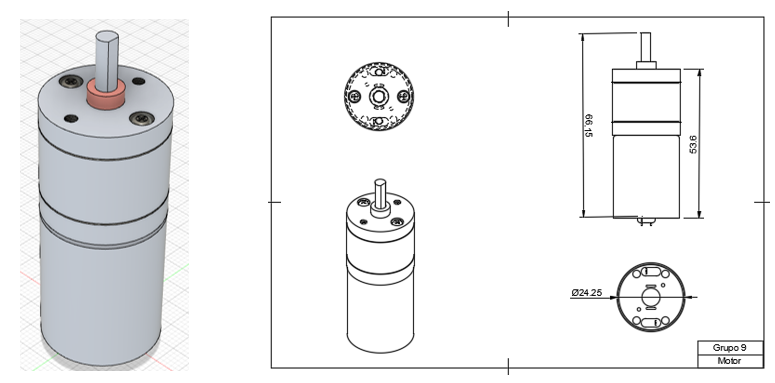
\includegraphics[width=0.6\textwidth]{./img/motor}
  \caption{Motores do robô}% 
\label{fig:motor}
\end{figure}

\item \emph{Rodas motriz e rodas giratórias:} O modelo do robô possui duas rodas motrizes e duas rodas giratórias. Foram utilizados designs já concebidos, sendo depois necessário adaptar às características do nosso robô (Figura \ref{fig:rodas-motriz} e Figura \ref{fig:rodas-gira}).
        %
    \begin{figure}[!h] 
\centering
    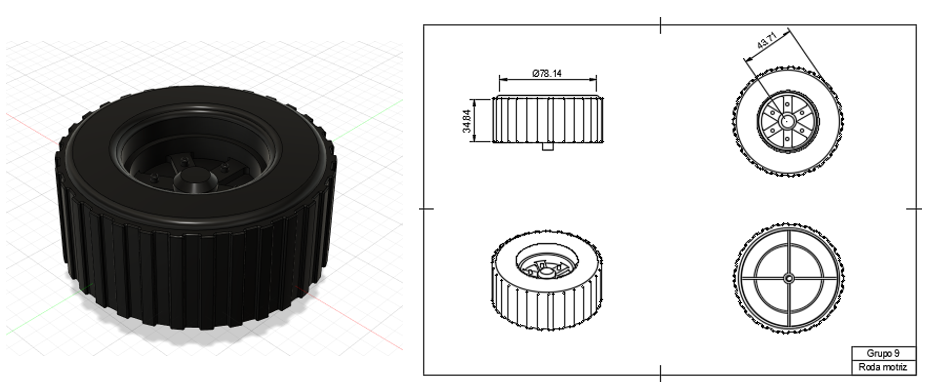
\includegraphics[width=0.6\textwidth]{./img/roda-motriz}
  \caption{Rodas motriz do robô}% 
\label{fig:rodas-motriz}
\end{figure}
        %
    \begin{figure}[!h] 
\centering
    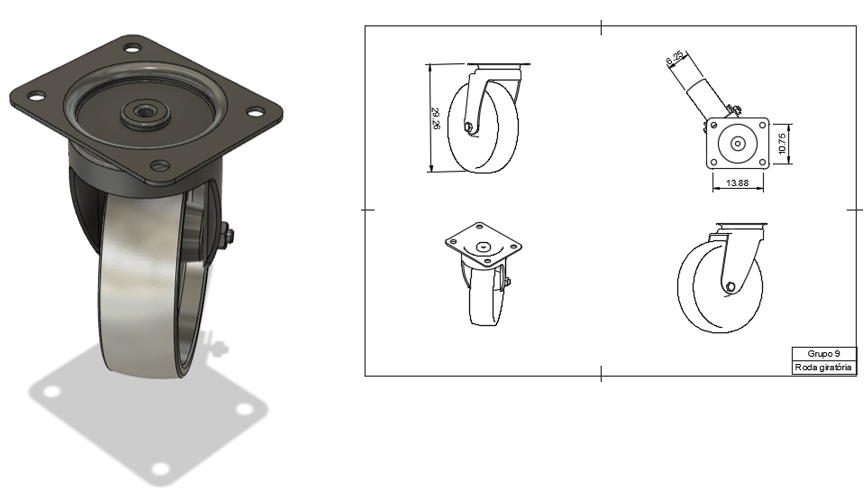
\includegraphics[width=0.6\textwidth]{./img/roda-gira}
  \caption{Rodas Giratórias do robô}% 
\label{fig:rodas-gira}
\end{figure}
\clearpage
\item \emph{Robô:} O robô é a junção de todas as peças mencionadas anteriormente (Figura \ref{fig:robo}).
        %
    \begin{figure}[!ht] 
\centering
    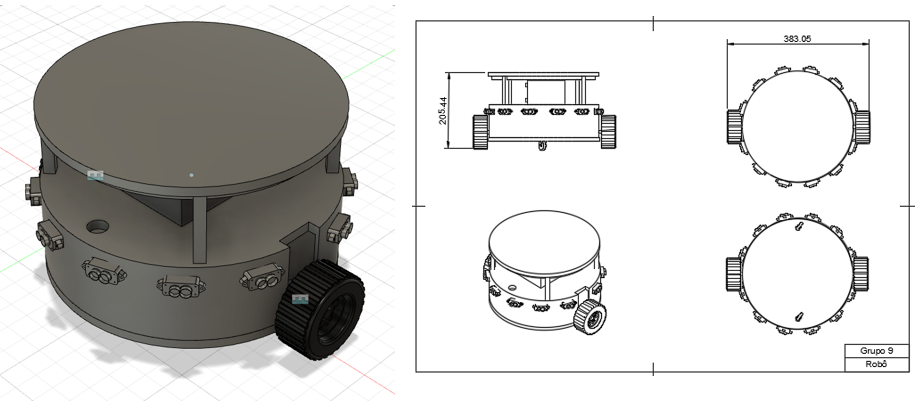
\includegraphics[width=0.7\textwidth]{./img/robo-total}
  \caption{Robô}% 
\label{fig:robo}
\end{figure}
\end{itemize}
\clearpage
\section{\textit{CoppeliaSim}}
\label{sec:coppelia}

O \textit{CoppeliaSim} é um simulador de robôs que usa um mecanismo de cinemática para cálculos de cinemática direta e inversa e várias bibliotecas de simulação. Modelos e cenários são construídos pela montagem de vários objetos numa estrutura hierárquica.

Após ter sido feito o modelo \textit{CAD}, há duas etapas para a criação de um projeto em \textit{CoppeliaSim}: criar um modelo físico e adaptar os scripts \textit{Matlab} para controlo do robô. Posto isto, desenvolveu-se um modelo físico simples para testar a física do robô, como é possível observar na Figura \ref{fig:robo-fisico}.

Para o desenvolvimento deste modelo, é necessário criar uma forma primitiva. Neste caso foi utilizada a forma de cilindro para desenvolver o corpo do robô e as duas rodas. De seguida é necessário adicionar motores e sensores. Para a criação e ajuste da localização de cada peça foram utilizadas as ferramentas \textit{Object/item shift} e \textit{Scene Object Properties}. Sendo que se trata de um modelo físico, foi adicionada física, através da ferramenta \textit{Show dynamic properties dialog} em \textit{Scene Object Properties} às rodas do modelo, atribuídos valores aos motores e através da ferramenta \textit{Show volume parameters}, foram configurados todos os sensores. 
%
    \begin{figure}[!h] 
\centering
    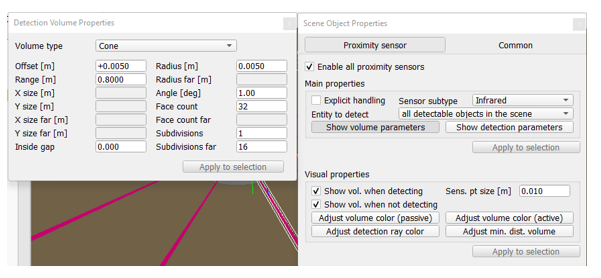
\includegraphics[width=0.8\textwidth]{./img/sens-prop}
  \caption{Propriedades dos sensores}% 
\label{fig:sensor-prop}
\end{figure}

        %
    \begin{figure}[!h] 
\centering
    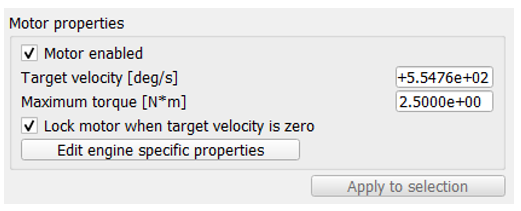
\includegraphics[width=0.6\textwidth]{./img/motor-prop}
  \caption{Propriedades dos motores}% 
\label{fig:motor-prop}
\end{figure}

        %
    \begin{figure}[!h] 
\centering
    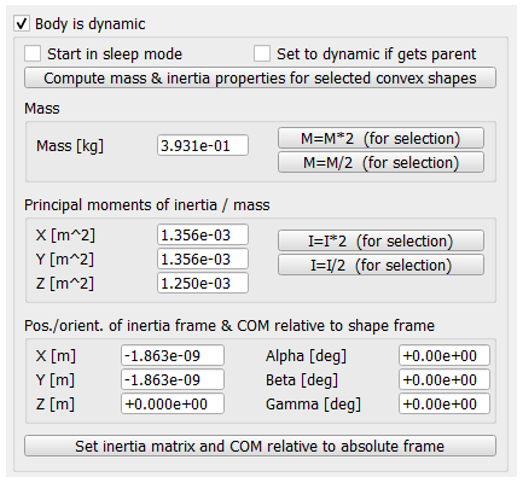
\includegraphics[width=0.6\textwidth]{./img/fisica-rodas}
  \caption{Física das Rodas}% 
\label{fig:rodas-fisica}
\end{figure}

Depois de testado o modelo físico, foi exportado o robô desenvolvido no \textit{Fusion} em formato \textit{.obj}, e inseriu-se este modelo no \textit{CoppeliaSim} sendo usado apenas como modelo gráfico, ou seja, serve apenas para visualizar. Isto pode ser feito através da ferramenta \textit{Common- Visibility} também em \textit{Scene Object Properties }. De seguida, ao robô obtido no \textit{CoppeliaSim}, adicionaram-se os sensores e foram colocados os elementos do robô de forma hierárquica para respeitar a física e comportar-se de acordo com o objetivo. Além disso foram utilizados cenários já desenvolvidos onde se colocou o robô e procederam-se testes para diversas situações. 
        %
    \begin{figure}[!h] 
\centering
    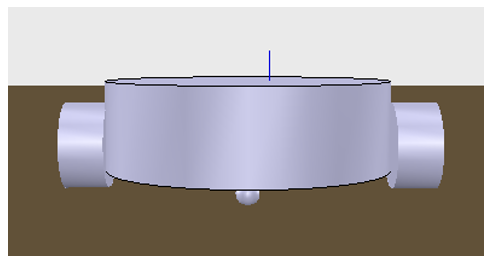
\includegraphics[width=0.7\textwidth]{./img/robo-copp}
  \caption{Modelo físico do robô}% 
\label{fig:robo-fisico}
\end{figure}

        %
    \begin{figure}[t] 
\centering
    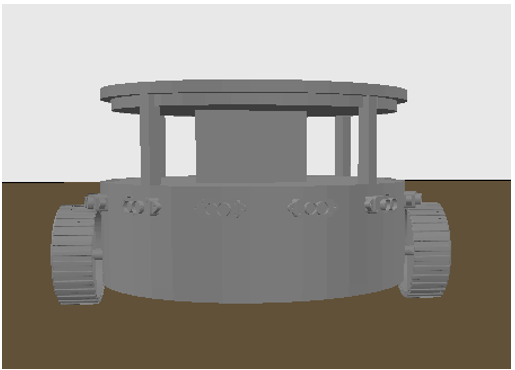
\includegraphics[width=0.7\textwidth]{./img/robo-copp-tot}
  \caption{Modelo total do robô}% 
\label{fig:robo-fisico-total}
\end{figure}
\section{Matlab}
\label{sec:matlab}

Por último, recorrendo ao código utilizado na unidade curricular de Sistemas Dinâmicos Não Lineares, foram efetuados alguns ajustes e alterações de acordo com as propriedades do robô desenvolvido.

No ficheiro program\_dyn\_EB\_tar\_obs, foram ajustados os parâmetros da velocidade do robô, taxa de decaimento, magnitude de repulsão e a magnitude do ruído, bem como foram acrescentadas/alteradas algumas partes do código. Uma vez que foi desenvolvido o controlo autónomo de dois robôs, ainda neste ficheiro, foram duplicadas as linhas de código de forma a controlar tanto o veículo 1 como o 2. De forma a ser possível visualizar graficamente dados relativos ao movimento do robô foram acrescentadas linhas de código com os plots. Todas estas alterações estão visíveis nas figuras seguintes.

Relativamente ao ficheiro RobDyn\_robot, alteraram-se as dimensões do robô e o número de sensores aplicados, de forma a corresponder ao robô desenvolvido. Para além disto, este ficheiro foi duplicado, RobDyn\_robot2, tendo sido nele alterados nomes de variáveis e funções uma vez que com a utilização de dois robôs, é necessário que estes tenham variáveis e funções com nomes distintos. Para além destes ficheiros, foi utilizado o ficheiro RobDyn\_simulation para tornar possível a conexão dos dois robôs no \textit{CoppeliaSim}.

De modo a testar o funcionamento do robô e validar a navegação autónoma foi testado um cenário variando algumas características do mesmo.
\clearpage

\lstinputlisting[language=matlab, firstline=31, lastline=45,caption={Objeto RobDyn\_robot},label=lst:robdyn-robot,
style=custom-matlab]{./listing/RobDyn_robot.m}
%
\lstinputlisting[language=matlab, firstline=31, lastline=45,caption={Objeto RobDyn\_robot2},label=lst:robdyn-robot2,
style=custom-matlab]{./listing/RobDyn_robot2.m}
%
\lstinputlisting[language=matlab, firstline=15, lastline=16,caption={Instanciação dos veículos},label=lst:insanc,
style=custom-matlab]{./listing/program_dyn_EB_tar_obs.m}
%
\lstinputlisting[language=matlab, firstline=144, lastline=223,caption={Código de navegação do veículo 1},label=lst:code,
style=custom-matlab]{./listing/program_dyn_EB_tar_obs.m}